\chapter{Anhang}
\label{ch:Anhang}

\begin{table}[htb]
\caption{Statistiken über Graph$_{5}$\label{tab:graph4}}
\vspace*{1em}
\centering

\bgroup
\def\arraystretch{1.3}%  1 is the default, change whatever you need

\begin{threeparttable}

\begin{tabular}[c]{ l  l  l | l  l}
	\hline
	\multicolumn{1}{c}{\textbf{Status}} & 
	\multicolumn{1}{c}{\textbf{Grad der Knoten}} & 
	\multicolumn{1}{c|}{\textbf{Knoten}} &
	\multicolumn{1}{c}{\textbf{Grad der Knoten}} & 
	\multicolumn{1}{c}{\textbf{Knoten}}\\
	
	\hline
		
	Vor der Reduktion & 0 & 0 &15  & 106 \\
	& 1 & 1 & 16&99 \\
	& 2 & 1 & 17& 84\\
	& 3 & 0 & 18& 66\\
	& 4 & 1 & 19& 39\\
	& 5 & 3 & 20& 27\\
	& 6 & 12 & 21& 16\\
	& 7 & 13 & 22& 18\\
	&  8& 17 & 23& 6\\
	&  9& 37 & 24& 3\\
	&  10& 65 & 25& 4\\
	&  11& 59 & 26& 5\\
	&  12& 101 & 27& 3\\
	&  13& 99 & 28& 1\\
	&  14& 114 & & \\
	
	\hline

	Nach der Reduktion & 0 & 0 & 6 & 18 \\
	& 1 & 0 & 7 & 11 \\
	& 2 & 55 & 8 & 8 \\
	& 3 & 59 & 9 & 0 \\
	& 4 & 46 & 10 & 0 \\
	& 5 & 41 & 11 & 1 \\
	
	\hline
	
\end{tabular}
\begin{tablenotes}\footnotesize
\item  Anzahl der Knoten pro Grad vor und nach der Reduktion für den besonderen Graphen der Nemhauser-Trotter - Kronenregel - Grad$_{1}$ - Reduktion
\end{tablenotes}

\end{threeparttable}

\egroup

\end{table}

Im Folgenden sind die Ergebnisse der restlichen Tests zu finden.

\begin{figure}[htb]
\centering
  	{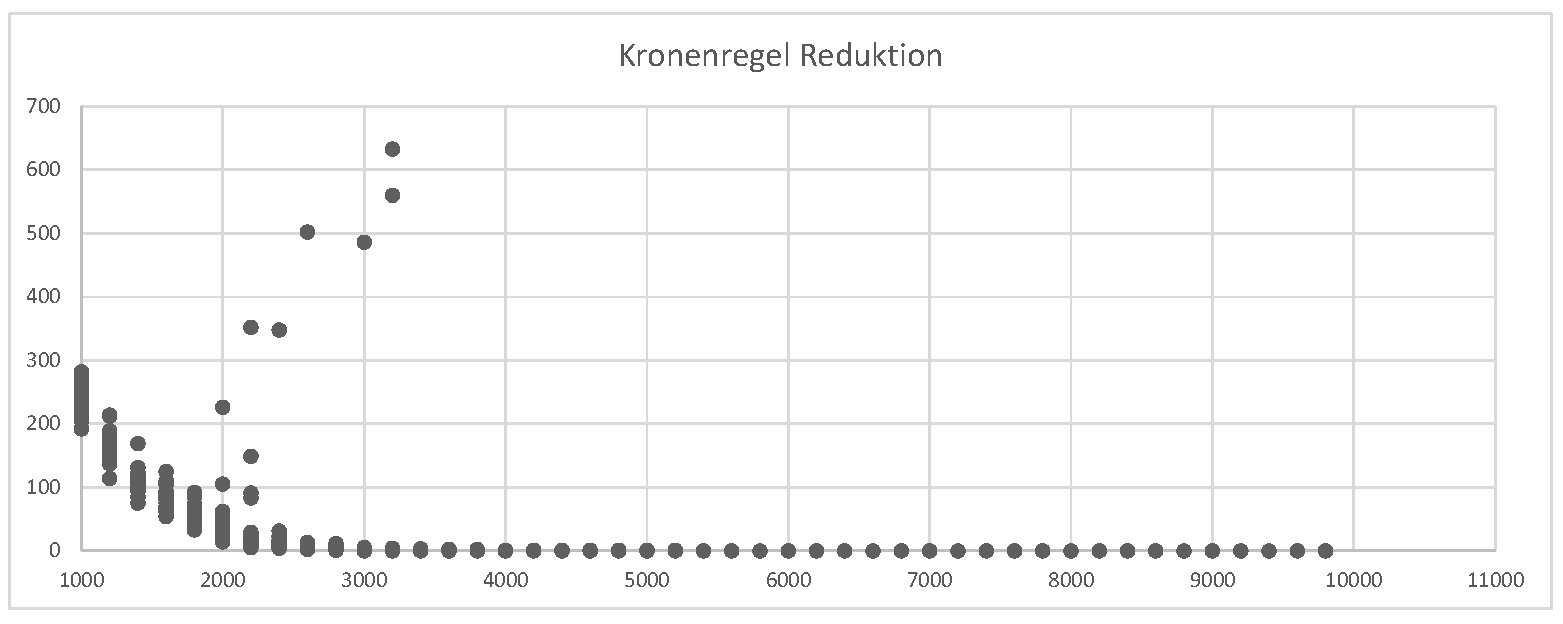
\includegraphics[width=\textwidth]{analysisCrown.pdf}}
	\caption{Anzahl der reduzierten Knoten pro Graph nach der Anwendung der Kronenregel\label{fig:crown}}
\centering
\end{figure}


\begin{figure}[htb]
\centering
  	{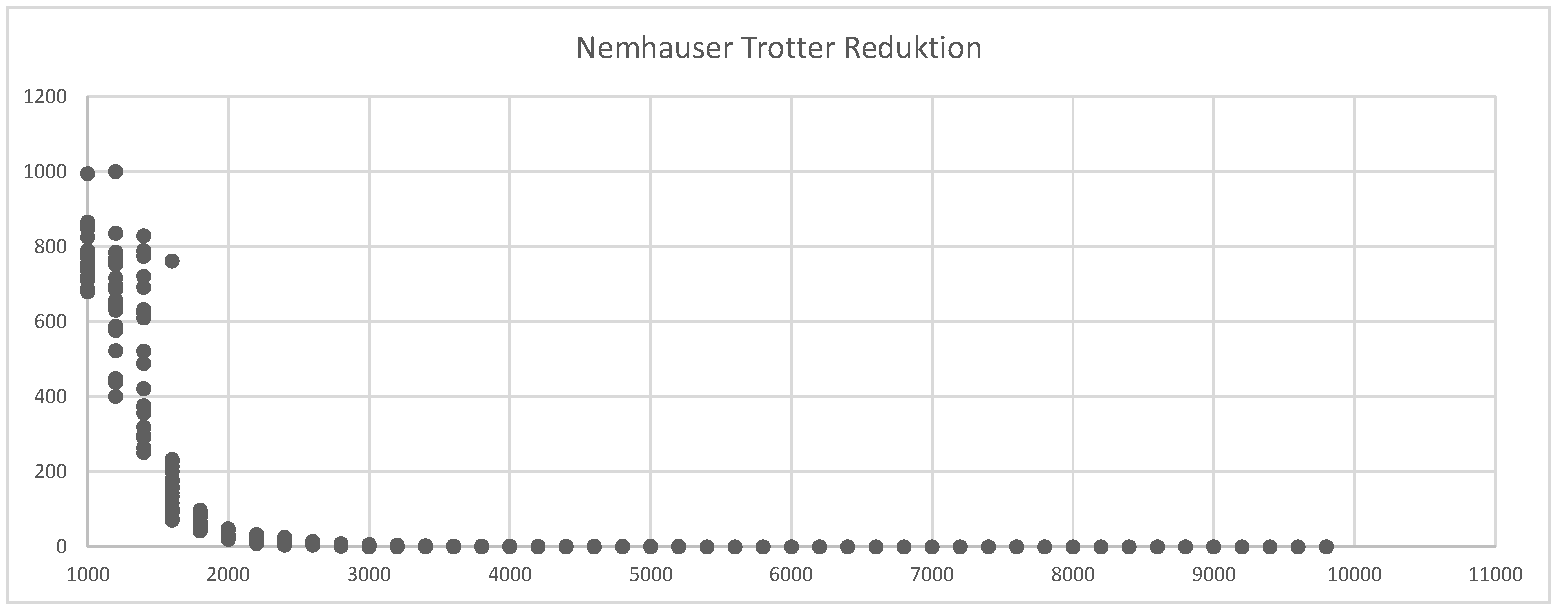
\includegraphics[width=\textwidth]{analysisTrottCrop.pdf}}
	\caption{Anzahl der reduzierten Knoten pro Graph nach der Anwendung der Nehmhauer-Trotter-Regel\label{fig:trott}}
\centering
\end{figure}


\begin{figure}[htb]
\centering
  	{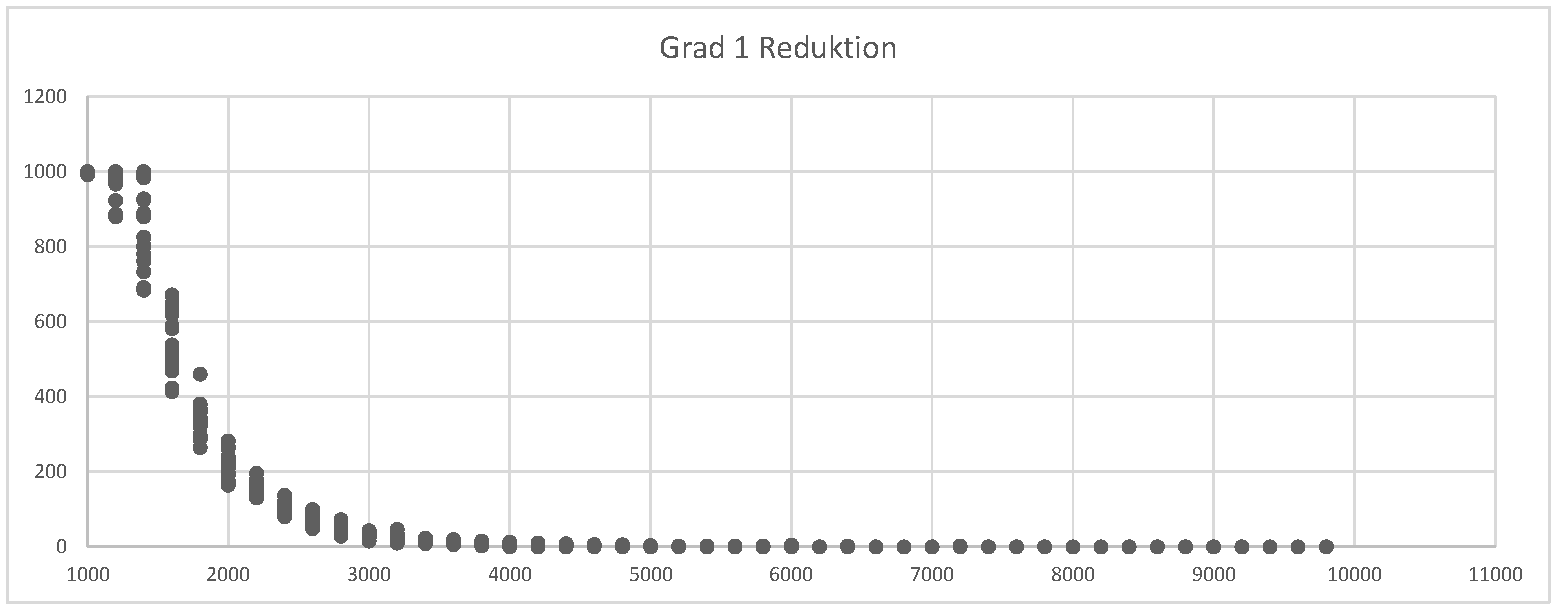
\includegraphics[width=\textwidth]{analysisOneCrop.pdf}}
	\caption{Anzahl der reduzierten Knoten pro Graph nach der Anwendung der Grad$_{1}$-Regel\label{fig:one}}
\centering
\end{figure}

